

\documentclass[oneside,20pt]{article}          % please do not change
\usepackage[b5paper]{geometry}	    % your paper can be easily printed on a4 or letter paper with enlargenment      
                                    % comment if you have problem with print     
\usepackage{amsfonts,amsmath,latexsym,amssymb}
\usepackage{graphicx}
%%% remove comment delimiter ('%') and specify parameters if required
%\usepackage[dvips]{graphics}

\begin{document}

%%% remove comment delimiter ('%') and select language if required
%\selectlanguage{spanish} 

\noindent 
\begin{center}
  \texttt{LABORATOR 6-- KEYLOGGER.}        
\end{center}

\section{KEYLOGGER}
\noindent                 
\\\\\
Keylogger-urile sunt unul dintre cele mai comune instrumente din cutia de instrumente a unui hacker. Sunt instrumente de baza a unui hacker și sunt ușor de făcut. În acest modul, vom învăța cum să codificăm un keylogger foarte eficient, dar precis.  Intai instalam biblioteca python de care avem nevoie: pip install pynput.
pynput: Acest lucru ne va ajuta să citim tastele pe măsură ce utilizatorul introduce siteuri sau parole.\\
Inregistrare: Aceasta va înregistra tastele într-un fișier pe care ulterior îl putem exfiltra prin mijloace adecvate.\\
Funcția definită aici (liniile 6-7) ia un argument care indică tasta apăsată de utilizator și îl conectează în fișier după ce îl convertește într-un șir.\\
A se vedea mai jos implementarea in python si testati la laborator acest cod!
\begin{center}
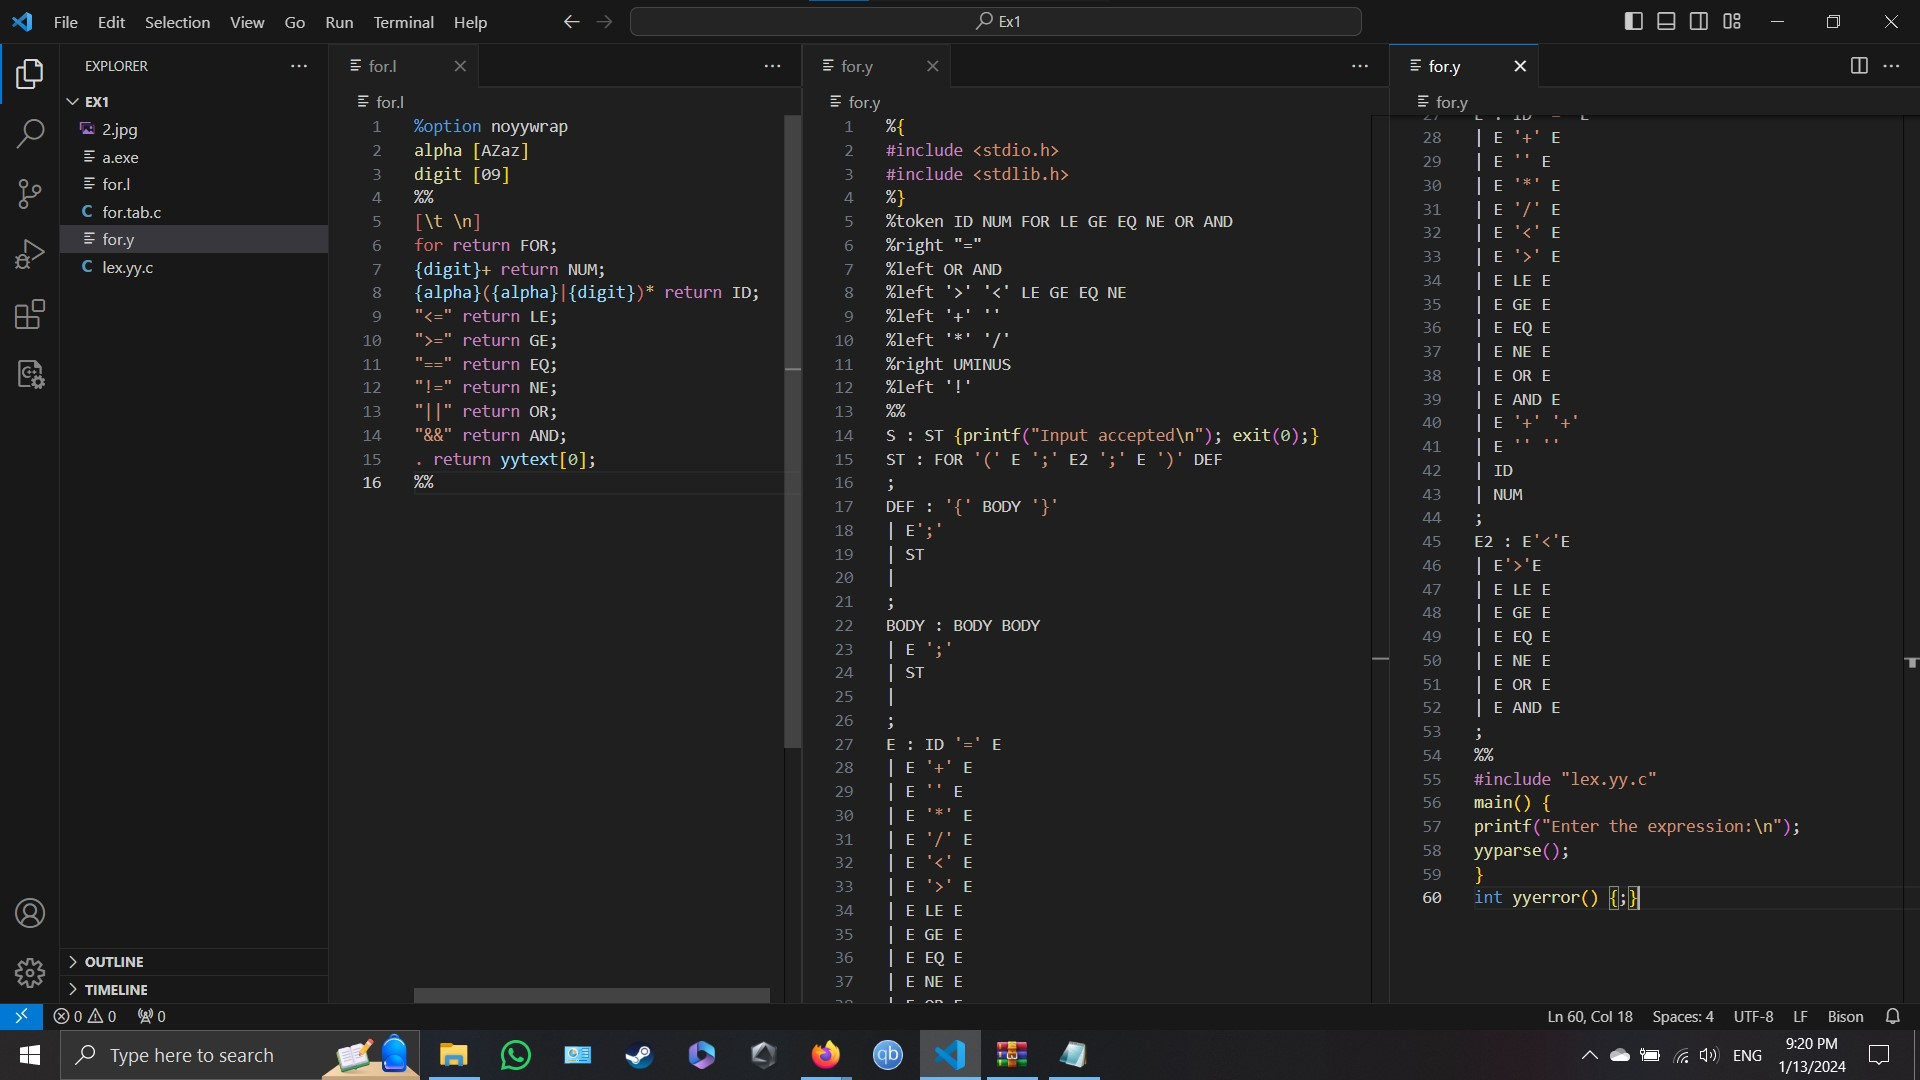
\includegraphics[height=3 cm]{1.png}
\end{center}

\section{Kick off a user from your wifi network}
Acest hack este o soluție la care probabil ați visat, mai ales dacă utilizați o
rețea care are o mulțime de alți utilizatori în ea. După cum probabil ați observat, există o anumită limită atunci când prin aceasta aavem trimitere și primire de date prin intermediul rețelei și al propriilor interfețe de rețea. Motivul pentru această limită este cantitatea de lățime de bandă pe care o aveți și dacă alți utilizatori nu ocupa  lățime de bandă, cu atât conexiunile dvs. vor fi mai rapide.
Când aveti toată lățimea de bandă, ar trebui să fie disponibilă pentru dvs., vă confruntați cu un DoS (Denial of
Service). De fapt, puteți forța un DoS către un alt utilizator căutând și manipulând serviciul wifi  al gazdei. Odată ce ați găsit deja acel serviciu, puteți face ca programul să se comporte într-un fel ceea ce nu ar trebui să facă, ceea ce va face ca gazda de la distanță să ocupe toate resursele disponibile și apoi il puteti scoate offline. Alternativ, puteți provoca și o inundație UDP, ceea ce se poate face
prin trimiterea unei cantități uriașe de pachete UDP către mai multe porturi de pe gazda la distanță a țintei dvs. Asta va
determina gazda să ignore orice aplicație care ascultă gazda respectivă și apoi să răspundă
cu un pachet care declara ICMP Destination Unreachable.
Pentru a face acest lucru, tot ce trebuie să faceți este să deschideți editorul de text și să introduceți următorul cod:
\begin{center}
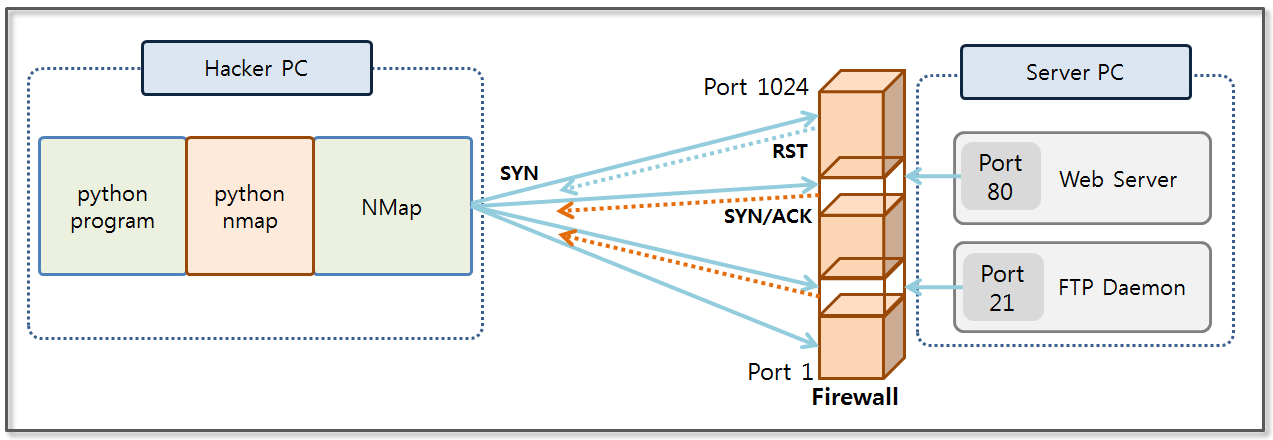
\includegraphics[height=5 cm]{2.png}
\end{center}
Salvați acest cod ca udpflood.py, apoi selectați toate opțiunile de fișier la salvare. Pentru a rula codul, rulati IDLE și apoi executați programul, care vă va solicita să introduceți toate celelalte informații de care aveti nevoie. Rețineți că acest hack este direcționat către un singur port, dar dacă doriți să le exploatați pe toate, alte 65.535 de porturi sunt disponibile.
\section{Wireless Attack: Dnspwn Attack}
Acest atac este creat prin utilizarea instrumentului airpwn, care este un cadru pentru injecția de pachete pentru
retele wireless 802.11. Acest instrument este creat pentru a asculta pachetele primite și apoi injectează conținut în
punctul de acces atunci când datele primite se potrivesc cu un model care este specificat în fișierul de configurare. Pentru ținta dumneavoastră, airpwn-ul tău arată și se comportă ca serverul cu care încearcă să comunice. Acest instrument
a fost creat mai întâi pentru a viza HTTP, dar poate fi folosit și pentru a exploata DNS.
În esență, folosirea unui atac dnspwn presupune atragerea țintei dvs. pentru a vizita o pagină web rău intenționată care
va instala programe malware la țintă prin descărcare sau pentru a falsifica un anumit site web pentru a-i fura
informații țintei dvs. Pentru a efectua acest atac, va trebui să aveți Backtrack sau Kali Linux
instalat în computer, precum și un adaptor de card wireless.
Urmați acești pași:\\
1. Setup your wireless monitor\\
Pentru a detecta activitatea wireless a țintei dvs., va trebui să vă configurați cardul wireless
adaptor la modul monitor. Pentru a face acest lucru, trageți airmon-ng din Kali Linux și apoi introduceți
următoarea comandă.\\
\begin{center}
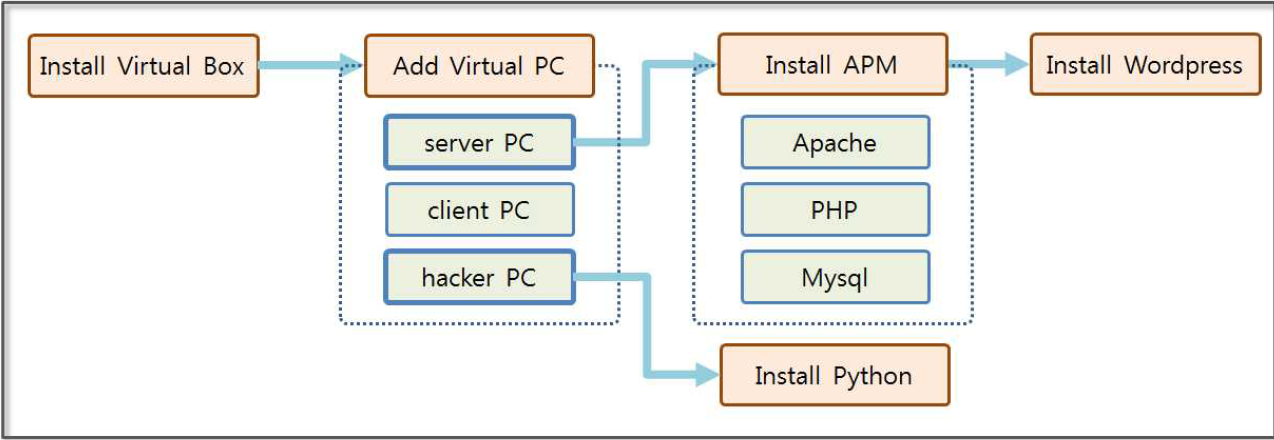
\includegraphics[height=0.5 cm]{3.png}
\end{center}
Acum, veți putea captura date chiar în rețeaua țintă.
Odată ce aveți un monitor în funcțiune, puteți începe să creați codul pentru atacul dvs.\\
2. Creați-vă codul.\\
Va trebui să utilizați modulul scapy pentru a efectua atacul dnspwn. La
acest moment, va trebui să investigati toate pachetele UDP care vin cu destinația portului 53
și apoi trimiteți pachetul cu funcția send response pe care o veți crea mai târziu.\\
\begin{center}
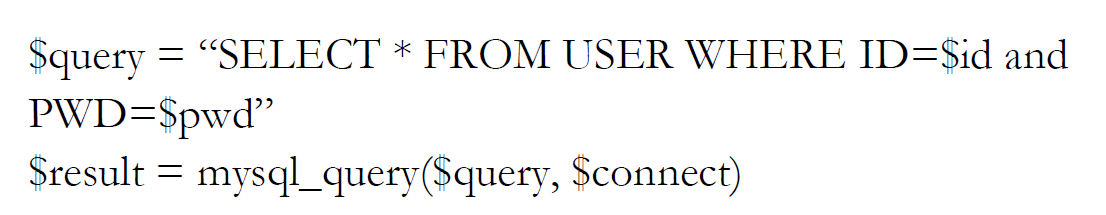
\includegraphics[height=2 cm]{4.png}
\end{center}
Acum că aveți modulul scapy, putem construi funcția care vă va permite
pentru a interpreta cererea pentru informațiile necesare și apoi a face injectarea răspunsului. Puteți
face acest lucru efectuând următorii pasi:\\
802.11 Frame – comutați indicatorul ”to-ds” la ”from-ds”, ceea ce îl va face să pară
ca și cum solicitările pe care le faceți provin de la punctul de acces\\
802.11 Frame – modificați adresele Mac ale destinației și sursei\\
Stratul IP – modificați adresele IP ale destinației și sursei\\
Stratul UDP – modificați porturile destinației și sursei\\
Stratul DNS - Introduceți steag ”răspuns”, apoi adăugați răspunsul pe care îl aveți
falsificat.\\
Modulul scape simplifică întregul proces eliminând multe detalii de care
nu trebuie să fii îngrijorat. Odată ce celelalte detalii au fost îndepărtate
prin scapy, puteți folosi următorul cod:
\begin{center}
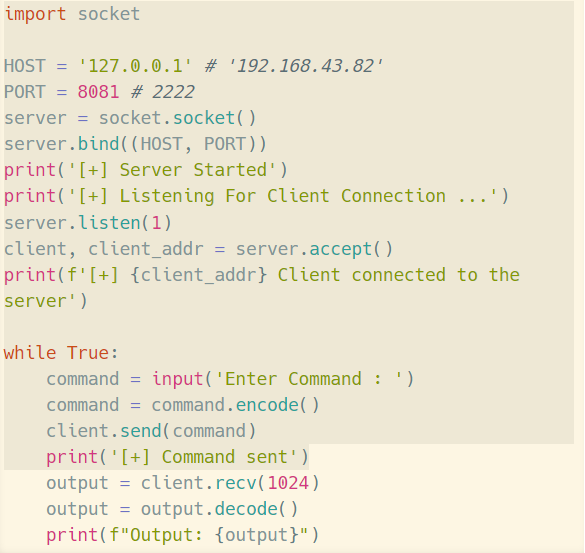
\includegraphics[height=5 cm]{5.png}
\end{center}
În acest moment, ai toate uneltele setate pentru atacul tău. Următorul pas este să creezi și să adaugi
raspunsul DNS:
\begin{center}
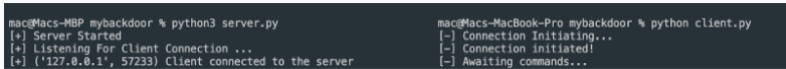
\includegraphics[height=3 cm]{6.png}
\end{center}
În cele din urmă, injectați răspunsul pe care l-ați falsificat:
\begin{center}
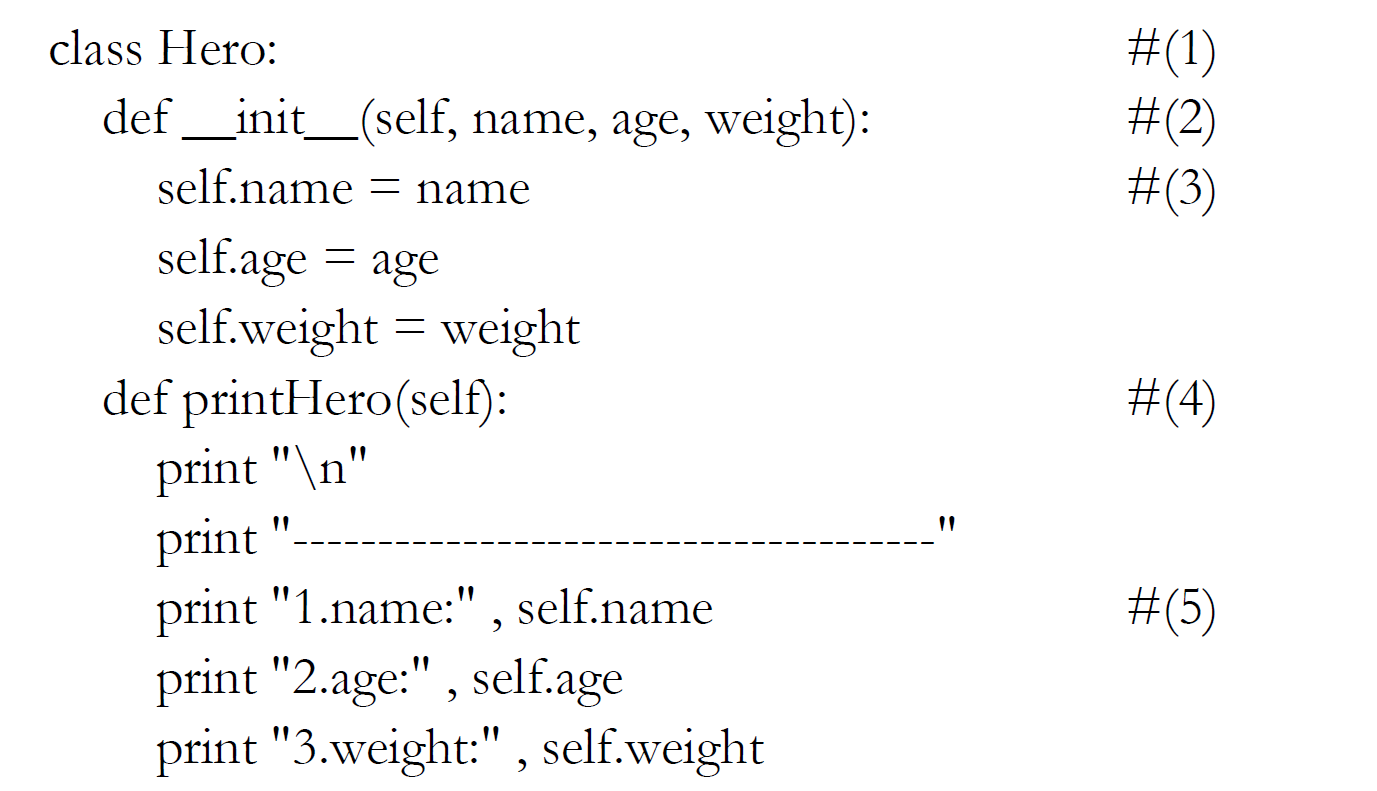
\includegraphics[height=0.5 cm]{7.png}
\end{center}
\section{Preveniți detectarea de către antivirus}
Un software antivirus este conceput pentru a detecta fișierele suspecte din sistemul dvs., cum ar fi virușii și
programe malware. Cu toate acestea, posibilitatea de a modifica conținutul unui malware vă va permite să ocoliți
detectarea antivirus.
În acest hack, veți putea învăța cum să creați un cod rău intenționat folosind un Kali Linux
componentă numită Metasploit. Acest program poate genera malware, dar majoritatea antivirusului
companiile pot recunoaște cu ușurință conținutul scris de acest software atunci când sunt lansate într-un
computer așa cum sunt scrise inițial. Pentru a crea un malware rezistent la antivirus, veți face acest lucru
 modificand malware-ul pe care îl veți crea folosind software-ul.
\section{Creați-vă programul mallware propriu}
Rulati Kali Linux și lansați un terminal. Rulați această comandă:
\begin{center}
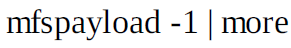
\includegraphics[height=0.5 cm]{21.png}
\end{center}
Mai mult, procedând astfel, se vor afișa vulnerabilitatile care sunt disponibile pentru utilizare, cum ar fi următoarele:
\begin{center}
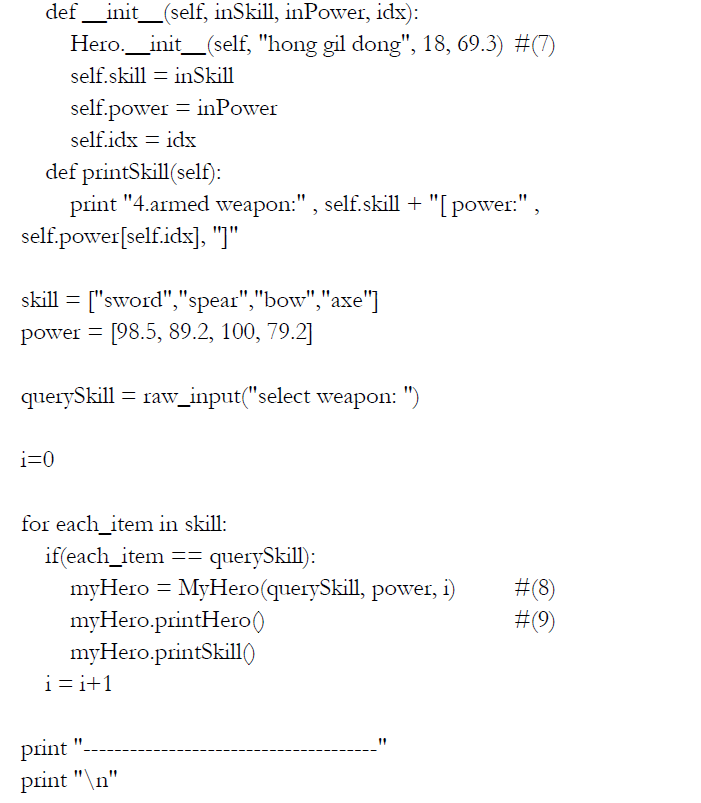
\includegraphics[height=4 cm]{8.png}
\end{center}
Dacă doriți să legați un shell pentru a crea un port, executați o comandă într-un port vizat,
și creați-vă propria telecomandă, introduceți aceste comenzi în terminalul Kali Linux:
\begin{center}
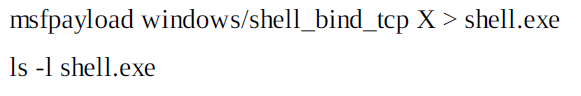
\includegraphics[height=0.5 cm]{8.1.png}
\end{center}

Veți obține următorul rezultat, care arată că Metasploit a creat un fișier executabil
numit shell.exe, care este malware-ul dvs.:
\begin{center}
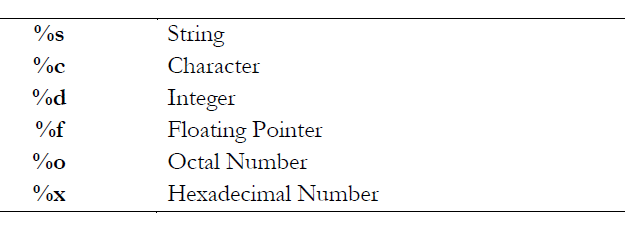
\includegraphics[height=2 cm]{9.png}
\end{center}
Desigur, orice software antivirus sensibil își va da seama că acesta este un fișier nesigur, care poate
compromite computerul unei ținte.
Testați-vă programul malware
Pentru a vedea că fișierul .exe pe care l-ați creat este recunoscut ca malware, transferați-l în alt
computer care are un program antivirus prin USB, e-mail sau trageți-l pe desktop prin copiere.
Aproape imediat, antivirusul instalat îl va prinde și îl va detecta astfel:
\begin{center}
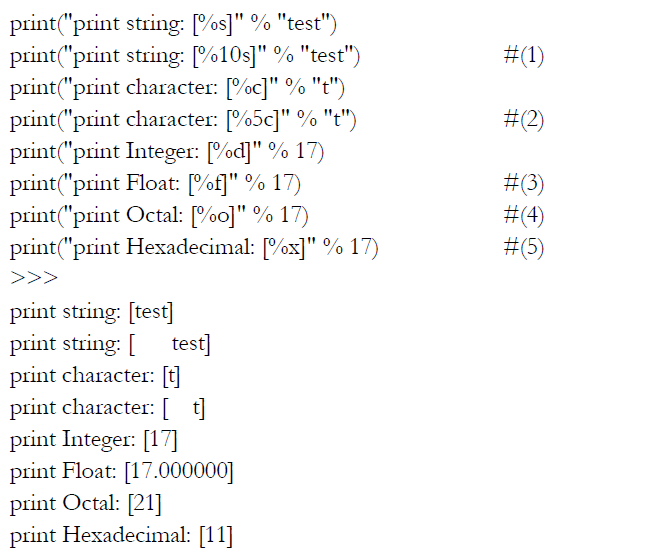
\includegraphics[height=4 cm]{10.png}
\end{center}
Acum, dacă intenționați să dezactivați software-ul antivirus și să rulați malware-ul, linia de comandă
va afișa ceva de genul acesta:
\begin{center}

\includegraphics[height=2 cm]{11.png}
\end{center}
Când se întâmplă acest lucru, puteți controla efectiv PC-ul cu Windows pe care este instalat malware-ul
folosind un alt computer.
Pentru a opri malware-ul, închideți fișierul shell.exe în Task Manager sau reporniți computerul.\\
Editați malware-ul folosind Python\\
Deoarece programul dvs. antivirus poate detecta malware-ul pe care l-ați creat, trebuie să editați malware-ul
codul pentru ca acesta să ocolească securitatea computerului dvs. Pentru a face asta, accesati Kali Linux și tastați
acest șir de comandă în terminal:
\begin{center}
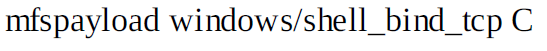
\includegraphics[height=1 cm]{20.png}
\end{center}
Veți vedea codul pentru exploit-ul pe care l-ați rulat anterior să fie în cod hexazecimal. Ce tu
trebuie să faceți este să compilați acest cod într-un fișier .exe. Pentru a face acest lucru, tot ce trebuie să faceți este să introduceți acest lucru
șir de comandă într-un terminal Kali Linux:
\begin{center}
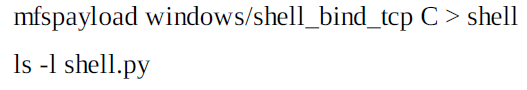
\includegraphics[height=1 cm]{9.1.png}
\end{center}
La introducerea acestui cod, Kali Linux va genera un fișier care arată astfel:
\begin{center}
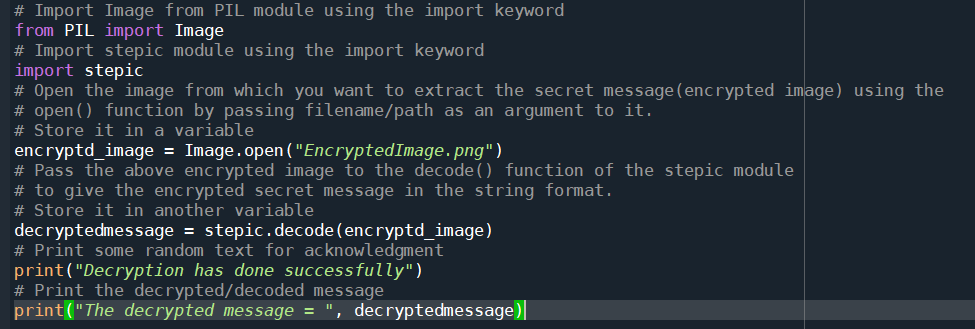
\includegraphics[height=2 cm]{12.png}
\end{center}
Acest cod este în limbaj C, ceea ce înseamnă că va trebui să adăugați câteva linii. Pentru a face asta, intrați
acest șir de comandă în terminalul Kali Linux: nano shell.py\\
Veți obține un editor de text cu acest cod:
\begin{center}
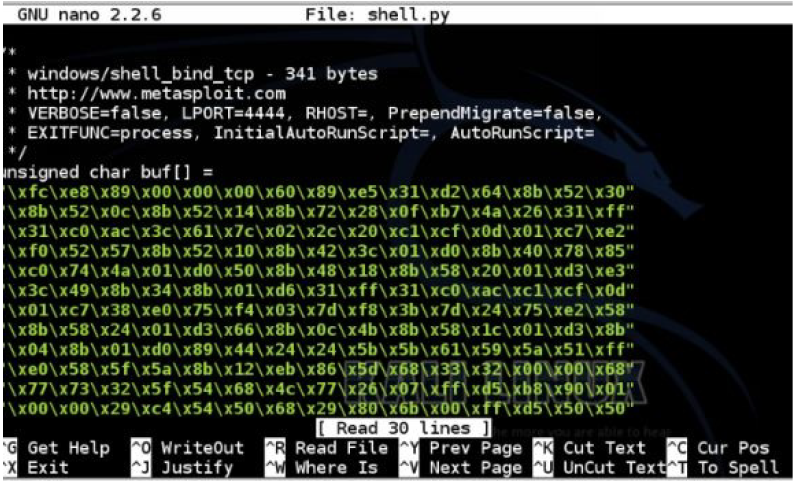
\includegraphics[height=4 cm]{13.png}
\end{center}
Importați codul bibliotecii sistemului care vă va permite să rulați programe C din Python. Pentru a face asta,
adăugați următoarea linie la începutul codului:
\begin{center}
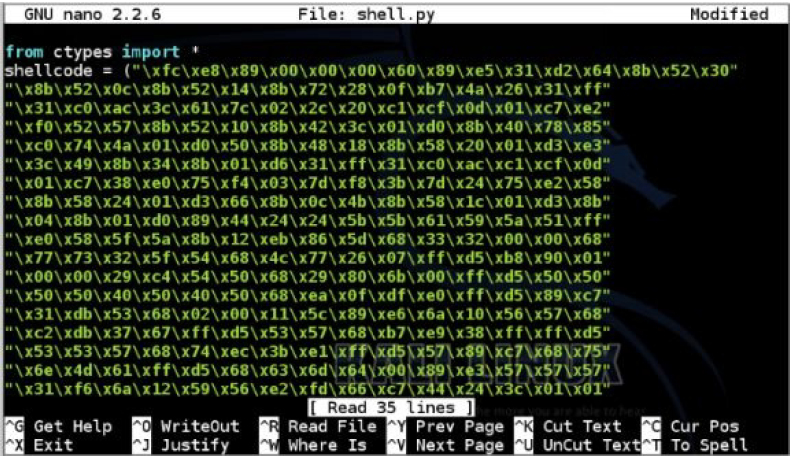
\includegraphics[height=4 cm]{14.png}
\end{center}
Derulați în jos și găsiți punctul și virgulă situat aproape de sfârșitul scriptului. Adăugați o paranteză de închidere. După ce faceți acest lucru, adăugați următoarele rânduri la sfârșitul codului:
\begin{center}
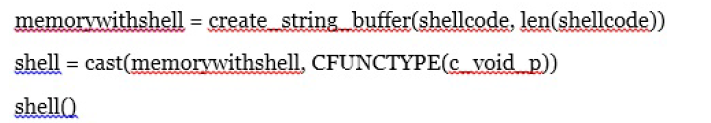
\includegraphics[height=1 cm]{15.png}
\end{center}
Ar trebui să vedeți acest lucru pe ecran după ce faceți acest lucru:
\begin{center}
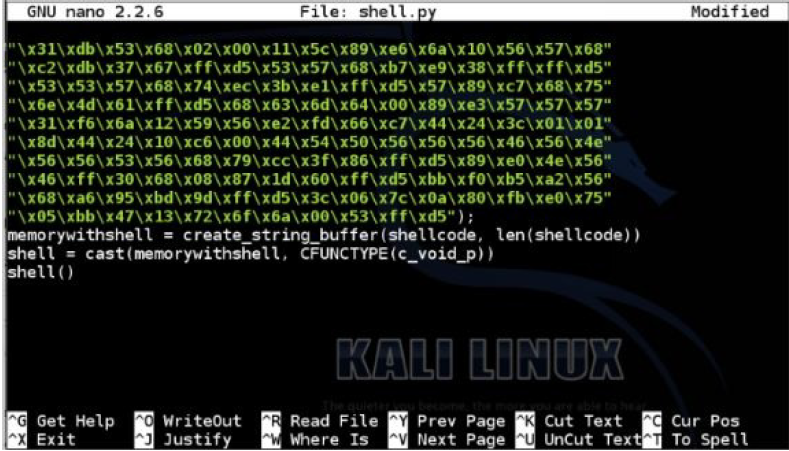
\includegraphics[height=3 cm]{16.png}
\end{center}
Pentru a salva fișierul, tastați Ctrl + X, apoi apăsați Y. Intră pentru a continua salvarea ta asupra fişierului modificat.\\
Compilați programul malware și rulați-l.
Pentru a rula malware-ul modificat, mai întâi va trebui să îl compilați. Pentru a face asta, în Command Prompt rulați acest șir de comandă:
\begin{center}
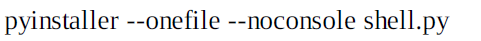
\includegraphics[height=1 cm]{17.png}
\end{center}
Aceasta va crea un folder nou numit ”dist”. Acest folder va avea malware modificat
în interiorul său numit shell.exe. Pentru a rula malware-ul, tot ce aveți nevoie este să deschideți folderul și să faceți dublu clic
în fișierul shell.exe.
Firewall-ul de protecție Windows ar putea bloca unele dintre caracteristicile programului, deoarece va încerca
conectivitatea la un server la distanță. Ocoliți acest lucru selectând Permiteți accesul. După ce faceți acest lucru, in Command Prompt rulați:
\begin{center}
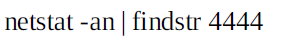
\includegraphics[height=1 cm]{18.png}
\end{center}
Aceasta va deschide un port de ascultare, care arată astfel:
\begin{center}
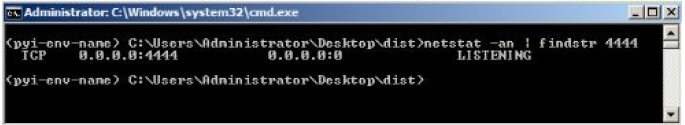
\includegraphics[height=2 cm]{19.png}
\end{center}
Pentru a opri ascultatorul, pur și simplu in Task Manager încheiați procesele numite shell.exe.
Verificați cu ajutorul antivirusului dacă malware-ul pe care tocmai l-ați creat mai poate fi detectat. Ar trebui sa
ocoliți majoritatea programelor antivirus cunoscute.

\section{Bibliografie}

https://www.askpython.com/python/examples/python-keylogger\\
 Steve Tale -Hacking with Python, 2017.


\end{document}
